% !TeX program = lualatex
\documentclass[12pt, fleqn, a4paper]{article}
\usepackage[top=2cm, bottom=2cm, left=3cm, right=1.5cm]{geometry}
\setlength{\parindent}{1cm}
\linespread{1.377388535031847}
\usepackage{luacode}

\begin{luacode*}
	function figurefix(word)
		tex.print("appendix")
	end
\end{luacode*}

\usepackage{fancyhdr}
\fancyhf{}
\fancyhead[C]{\thepage}
\renewcommand{\headrulewidth}{0pt}
\pagestyle{fancy}

\fancypagestyle{plain}{%
  \fancyhf{}
  \renewcommand{\headrulewidth}{0pt}
  \fancyhead[C]{\thepage}
}

\usepackage{listofitems}
\newcommand\substr[3]{%
  \setsepchar{#2}%
  \readlist\parsedinput{#1}%
  \foreachitem\x\in\parsedinput{%
    \ifnum\xcnt=1\else#3\fi\x%
  }%
}


\usepackage{pdfpages}
\usepackage{fontspec}
\defaultfontfeatures{Mapping=tex-text,Scale=MatchLowercase}
\setmainfont{Times New Roman}
\setmonofont{Noto Sans Mono}
\usepackage{indentfirst}
\usepackage{polyglossia}
\usepackage{changepage}
\usepackage[fontsize=12.5pt]{scrextend}
\usepackage{markdown}
\usepackage{etoolbox}
%\usepackage{hyperref,url}
\usepackage{natbib}
\newcounter{bibcount}

\makeatletter
\patchcmd{\@lbibitem}{\item[}{\item[\hfil\stepcounter{bibcount}{\thebibcount.}}{}{}
\setlength{\bibhang}{2\parindent}
\renewcommand\NAT@bibsetup%
   [1]{\setlength{\leftmargin}{\bibhang}\setlength{\itemindent}{-\parindent}%
       \setlength{\itemsep}{\bibsep}\setlength{\parsep}{\z@}}
\makeatother
\bibliographystyle{agsm}


% Language setting
\setdefaultlanguage{english}

\usepackage{enumitem}
\setlist[enumerate]{label*=\arabic*.}
\AddToHook{cmd/section/before}{\clearpage}

\usepackage{minted}
\setminted[python]{frame=single}

\usepackage{lipsum}
\usepackage{titlesec}
\renewcommand{\thesection}{\arabic{section}.{}}
\renewcommand{\thesubsection}{\arabic{section}.\arabic{subsection}.{}}
\renewcommand{\thesubsubsection}{\arabic{section}.\arabic{subsection}.\arabic{subsubsection}.{}}

\usepackage{tocloft}
\usepackage{float}
\renewcommand{\cftsecleader}{\cftdotfill{\cftdotsep}} 

\usepackage{sectsty}
\newcommand{\HeaderSize}{\fontsize{14}{15}\selectfont\MakeUppercase}
\sectionfont{\HeaderSize}

\usepackage{chngcntr}
\counterwithin{figure}{section}

\usepackage{xstring}
\def\FixCaptionLabel#1{%
  \IfSubStr{#1}{.}{%
	\StrSubstitute[1]{#1}{.}{}}{#1}}


\newcommand{\figurefix}[1]{\directlua{figurefix("#1")}}

\begin{luacode}
function fixTableNumbering(input)
    out = string.gsub(input, "%.", "", 1)
    tex.print(out)
end
\end{luacode}

\newcommand{\fixtablenumbering}[1]{\directlua{fixTableNumbering("#1")}}

\usepackage{caption}
% Configure table caption style
\DeclareCaptionFormat{myformat}{\hfill#1#2\\\textbf{#3}}
\DeclareCaptionLabelFormat{mylabelformat}{#1 #2}
\captionsetup[table]{format=myformat, labelsep=quad, singlelinecheck=false, justification=centering, labelformat=mylabelformat}

\usepackage{subcaption}
\DeclareCaptionLabelFormat{custom}
{%
	\FixCaptionLabel{#2}. #1.
}

\DeclareCaptionLabelFormat{customappendix}
{
	#2. \figurefix{#1}
}



% Separator style
\DeclareCaptionLabelSeparator{custom}{ }

% Caption format    
\DeclareCaptionFormat{custom}
{%
	#1#2\textbf{#3}
}

\DeclareCaptionFormat{customappendix}
{%
	#2#1  \\ \textbf{#3}
}


\captionsetup
{
    format=custom,%
    labelformat=custom,%
    labelsep=custom
}


\newcommand\signature[2]{% Name; Department
\noindent\begin{minipage}{5cm}
    \noindent\vspace{3cm}\par
    \noindent\rule{5cm}{1pt}\par
    \noindent\textbf{#1}\par
    \noindent#2%
\end{minipage}}

\newcommand\conformationsignature[2]{
\begin{table}[h]
    \begin{tabular}{p{7cm}}
      \\
    \end{tabular}
    \begin{tabular}{p{3cm}}
      \\\hline
    #1 
    \end{tabular}
    \begin{tabular}{p{4cm}}
      \\\hline
    #2 
    \end{tabular}
\end{table}
}

\newcommand\insertdate[1][\today]{\vfill\begin{flushright}#1\end{flushright}}
\usepackage{csquotes}
\usepackage{plantuml}
\usepackage{soul}
\usepackage{xcolor}
\definecolor{light-gray}{gray}{0.95}
\newcommand{\ctext}[3][RGB]{%
  \begingroup
  \definecolor{hlcolor}{#1}{#2}\sethlcolor{hlcolor}%
  \hl{#3}%
  \endgroup
}

\newcommand{\codeline}[1]{\ctext[RGB]{236,236,236}{#1}}
\newcommand{\codeword}[1]{\colorbox{light-gray}{\texttt{#1}}}
\newcommand{\cw}[1]{\colorbox{light-gray}{\texttt{#1}}}
\newcommand{\boldword}[1]{\textbf{#1}}

\begin{luacode*}
	function split(inputstr, sep)
	        if sep == nil then
	                sep = "%s"
	        end
	        local t={}
	        for str in string.gmatch(inputstr, "([^"..sep.."]+)") do
	                table.insert(t, str)
	        end
	        return t
	end

	function boldenfirstword(line)
		local words = split(line, " ")
		local fword = words[1]
		table.remove(words, 1)
		tex.print("\\textbf{"..fword.."} "..table.concat(words," "))
	end
\end{luacode*}

% declare a wrapper in TeX
\newcommand{\boldenfirstword}[1]{\directlua{boldenfirstword("#1")}}

\usepackage{datatool}
\newcommand{\sortitem}[1]{%
  \DTLnewrow{list}% Create a new entry
  \DTLnewdbentry{list}{description}{\boldenfirstword{#1}}% Add entry as description
}

\newenvironment{sortedlist}{%
  \DTLifdbexists{list}{\DTLcleardb{list}}{\DTLnewdb{list}}% Create new/discard old list
}{%
  \DTLsort{description}{list}% Sort list
  \begin{itemize}%
    \DTLforeach*{list}{\theDesc=description}{%
\item[] \theDesc}% Print each item
  \end{itemize}%
}

\setlength{\cftsubsubsecindent}{\cftsubsecindent}
%\setlength{\cftsubsubsecnumwidth}{1.25cm}
%\setlength{\cftsubsecnumwidth}{1.25cm}

\usepackage[toc,page]{appendix}
\usepackage{listings}
\usepackage{fancyvrb}
\usepackage{booktabs}
\usepackage[fleqn]{nccmath}
\usepackage[framemethod=tikz]{mdframed}



\lstset{
breaklines=true,
breakatwhitespace=false,
xleftmargin=1em,
%frame=single,
%numbers=left,
numbersep=5pt,
}

\newcommand\mylstcaption{}

\mdfdefinestyle{mymdstyle}{
hidealllines=true,
%middleextra={
%  \node[anchor=west] at (O|-P)
%    {\lstlistingname~\thelstlisting\  (Cont.):~\mylstcaption};},
%secondextra={
%  \node[anchor=west] at (O|-P)
%    {\lstlistingname~\thelstlisting\  (Cont.):~\mylstcaption};},
splittopskip=2\baselineskip
}

\surroundwithmdframed[style=mymdstyle]{lstlisting}
\newmdenv[style=mymdstyle]{mdlisting}

\usepackage{amsmath}
\usepackage{cleveref}

% Lua code to modify the label
\begin{luacode}
function fixDots(input)
    out = string.gsub(input, "%.", "", 1)
    tex.print(out)
end
\end{luacode}

\newcommand{\fixdots}[1]{\directlua{fixDots("#1")}}
\crefformat{figure}{Figure ~\fixdots{#2#1#3}}
%\crefformat{table}{Table #2#1#3}
\renewcommand*\descriptionlabel[1]{\hspace\leftmargin$#1$}



\begin{document}
%\includepdf[pages={1,2,3,4}]{final.pdf}
\setcounter{page}{5}


\renewcommand{\cfttoctitlefont}{\hfill\Large\bf}
\renewcommand{\cftaftertoctitle}{\hfill\hfill}
\let\oldcontentsname\contentsname
\renewcommand{\contentsname}{ \HeaderSize \hfill \HeaderSize \oldcontentsname}
\renewcommand{\cftsecfont}{\mdseries\scshape\sffamily}
\renewcommand{\cftsecpagefont}{\mdseries\scshape\sffamily}


\setlength\cftbeforesecskip{1pt}

\tableofcontents
\newpage

\addcontentsline{toc}{section}{List Of Used Abbreviations}
\section*{\centering List Of Used Abbreviations}
\begin{adjustwidth}{113pt}{43pt}
	\begin{sortedlist}
		\sortitem{VPN - Virtual Private Network}
		\sortitem{GFW - Great Firewall of China}
		\sortitem{DPI - Deep Packet Inspection}
		\sortitem{TCB - TCP Control Block}
		\sortitem{TCP - Transmission Control Protocol}
    \sortitem{HTTPS - Hypertext Transfer Protocol Secure}
    \sortitem{SSL - Secure Sockets Layer}
    \sortitem{ISP - Internet Service Provider}
    \sortitem{IP - Internet Protocol}
    \sortitem{TCP - Transmission Control Protocol}
    \sortitem{UDP - User Datagram Protocol}
    \sortitem{TLS - Transport Security Layer}
    \sortitem{ML - Machine Learning}
    \sortitem{AI - Artificial Intelligence}
    \sortitem{SSH - Secure Shell}
    \sortitem{VM - Virtual Machine}
    \sortitem{NAT - Network Address Translation}
	\end{sortedlist}
\end{adjustwidth}
\addcontentsline{toc}{section}{Introductions}
\section*{\centering Introduction}
In an time when digital communication plays a fairly important role in modern socienty, ensuring the confidentiality and integrity of network communications has become crucial. The arrival of virtual private networks (VPNs) as a way of securing and privatizing digital communications on the publicly used Internet has been a significant development in this direction. Because of the ever growing popularity of virtual private networks, government agencies and corporate network administrators have ever so increased their efforts to identify and block these encrypted connections. The result has been, what one may call, an arms race between organizations seeking to monitor, control, or censor Internet traffic and VPN service providers competing for the privacy of their users. The implementation of VPN obfuscation, an advanced collection of technologies capable of disguising VPN traffic as routine Internet operations, is central to this dispute. This obfuscation allows free access to the global digital landscape.

Initially, VPNs were implemented as just a way to establish secure network connections across the insecure infrastructure of the public Internet. However, the use of VPN technology eventually grown ouside of the scope of corporate applications. Privacy oriented users are increasingly adopting virtual private networks for their own benefit, due to the potential for enhanced privacy, circumvention of surveillance, circumvention of content location based restrictions, and protection against cyber threats. In response, efforts to undermine the effectiveness of virtual private networks have increased. These initiatives include corporate firewall policies, government censorship initiatives such as China's Great Firewall, and anti-VPN measures implemented by content providers \citep{DPL}.

The gradual and yet noticable proliferation of anti-VPN initiatives has sparked the emergence of a complex area of cybersecurity that uses data packet signatures to distinguish VPN connections. In response, the VPN obfuscation movement has developed a number of countermeasures. As a recent example, we have the Geneva algorithm which employs genetic algorithms to generate dynamic, packet-
manipulation-based evasion strategies, providing a new take on Deep Packet Inspection (DPI) evasion \citep{Geneva}.

Steganography can also be utilized in VPN obfuscation. This method provides a way around DPI systems by embedding VPN traffic inside regular data streams. Steganography enables regular web traffic, like audio or video streams, to conceal VPN packets, making it difficult for DPI tools to discern between encrypted and regular traffic \citep{Stega}. The effectiveness and subtlety of this method are assessed, offering insights into its limitations and useful applications in different network environments.

Another way of obfuscating VPN traffic is through the application of port switching. To avoid detection, a VPN server is configured to use non-standard ports, which can assist in getting around simple DPI systems that keep an eye on popular VPN ports. 

Another way of providing VPN obfuscation is the integration of encrypted proxy tunneling software like Shadowsocks and Stunnel. It can be used to make VPN traffic look like HTTPS traffic \citep{Shadowsocks}. 

All of these methods, excluding port switching, bring with them a trade-off of in connection speed and throughput, 
though of varying degrees.

The thesis begins with an overview of VPN technology and then describes the various use cases for VPNs as well as the fundamental principles underlying their operation. It then describes the techniques used to detect VPN traffic. The following is a comprehensive examination of various obfuscation methods and their adaptation to evolving VPN traffic detection strategies. The goal of this analysis is to provide insight into VPN detection methodologies and obfuscation techniques through experimentation, literature analysis, qualitative assessment, and technical proficiency in the process developing a methodology by which one can consider selecting an obfuscation method in real-life scenarios. The bulk of the experimentation was conducted utilizing a virtual networking topology with the prime VPN being OpenVPN and ndpi being used as the DPI system. The questions this thesis aims to answer are as follows:
\begin{itemize}
  \item Which of the selected VPN obfuscatory methods are capable evading detection of the nDPI deep-packet inspection system within the provided virtual network topology?
  \item How effective these methods are in terms of selected evaluation criteria?
  \item Which method to choose in a real-life scenario?
\end{itemize}

\section{Literature}
For the purposes of gaining insight into the topic of VPN obfuscation an extensive dive and analysis was conducted into the topic of VPNs, DPI and protocol obfuscation. Many related sources and research publications were found, though it may be noted that none of the research results found were of a similar nature to my own topic. Much of the research, was of a more focused nature, typically centering around a more narrow topic. None of them took a comparative approach to the VPN obfuscation methods. In addition, they approached the topic from a different perspective. The perspective of general data hiding, not taking VPNs into consideration, some examples being \cite{Geneva}, \cite{Stega} and \cite{symtcp} where there is no explicit mention of VPNs. In addition, many research publications were aimed towards the opposite, with the goal of developing progressively new ways of detecting VPN traffic instead of hiding it, examples of thing being \cite{detection1}, \cite{detection2} and \cite{detection3}.

\subsection{Search Strategy}
The process of finding source of literature was incremental and partially iterative in its nature. At first, a list of topic specific terms and keywords was compiled: Deep packet inspection, network traffic analysis, censorship circumvention. 
With these keywords, a number of initial sources were found, those most prominently included: \cite{Geneva}, \cite{gohop} and \cite{DPL}.

Based on the found literature sources, a more clear understanding of the topic and its terminology was garnered. Accordingly, an extended list terms and keyword was compiled which now included: steganography, packet fragmentation, traffic manipulation, network security, Obfsproxy. 
This process was then again repeated until an adequate understanding of the topic was achieved.

\subsection{Literature Repository Selection}
In order to find the literature a number of digital libraries were utilized based on the degree of relevance in relation to the topics of computer science, networking and software engineering. The most prominent of those repositoiries being:
\begin{itemize}
  \item Research Gate
  \item IEEE Xplore
  \item ArXiv
  \item ACM Digital Library
  \item Springer Link
  \item Dergi Park
\end{itemize}
In some exceptional cases, more unoffical sources were used, for example, jouralist articles or website documentation. This applied for cases like \cite{Shadowsocks} and \cite{openvpn2} where the most reliable source of information for how Shadowsocks and OpenVPN work came from website documentation.
\subsection{Exclusion criteria}
For the systematic review of literature relating to VPN obfuscation, Deep Packet Inspection, and protocol obfuscation, certain exclusion criterias were employed to ensure the relevance and validity of the chosen sources. These criteria were used in filtering out literature that did not directly contribute to the understanding of the topic or meet the requirements. The used exclusion criteria are as so:
\begin{itemize}
\item \textbf{Non-Academic Sources:} Sources lacking peer-review or not published in recognized academic journals or conferences were excluded to the utmost degree. This includes blog posts, non-reviewed whitepapers, and informal publications. Though still, some non-academic sources were used when absolutely needed.
\item \textbf{Irrelevant Topics:} Literature that did not directly address VPNs, VPN obfuscation, DPI, or protocol obfuscation was excluded. This encompasses studies focused solely on broader topics of corporate network security or general VPN usage. Though, to be clear, papers that provide in some way a detailed technical explanation on how protocols, VPNs or DPI were, in certain cases, were included. 
\item \textbf{Language Constraints:} Sources not available in English were excluded.
\item \textbf{Duplicate Studies:} In cases where multiple publications reporting the same information or research, only the most comprehensive or recent version was included.
\item \textbf{Geographical Irrelevance:} Studies focusing on region specific VPN usage or censorship practices, which are not applicable or relevant to the broader context of global VPN obfuscation, were excluded.
\item \textbf{Technical Inapplicability:} Research that focuses on obsolete or rarely used VPN protocols or technologies was excluded, to concentrate on methods and findings relevant to current practices.
\end{itemize}
These exclusion criteria were applied to make sure the collection of literature was focused and relevant. The criteria were developed to strike a balance between inclusiveness and specificity, therefore providing a comprehensive overview of the current state of research in VPN obfuscation, DPI, and protocol obfuscation.


\subsection{Found literature}
As mentioned before, a number of sources relating to VPNs, protocol obfuscation and DPI were successfully found. Though all of these sources differ in their goal from this thesis. None of them perform a wide comparative review and analysis for VPN obfuscation methods. The found literature is used as a source of information, from which a comprehensive overview of VPN obfuscation is synthesized
\subsubsection{VPN related literature}
The found literature addressing VPNs is quite diverse. Covering various topics from technical implementation to traffic identification and obfuscation. Here is a general overview of the key literature in this area:
\begin{itemize}
  \item \textbf{OpenVPN Traffic Identification:} \cite{openvpn} in their work titled "OpenVPN Traffic Identification Using Traffic Fingerprints and Statistical Characteristics" provides a good general overview on how OpenVPN traffic could be identified. This information is critical towards understanding the characteristics of VPN traffic and how DPI can go about detecting it.
  \item \textbf{SSL VPN Advanteges:} The benefits of SSL based VPNs is discussed in-depth by \cite{sslvpn} and this work highlights certain features and benefits of SSL VPNs, which are critical for secure and remote access.
  \item \textbf{General VPN overview:} a basic definition and understanding of VPNs is provided by \cite{whatvpn} helping to establish a baseline border between data obfuscation and VPN obfuscation.
  \item \textbf{Tor and VPNs:} The intersection of Tor and VPNs is discussed in the chapter "Tor Relays, Bridges, and Obfsproxy" by \cite{bridges}. The chapter provides a fairly well-rounded understanding of how Tor and VPNs can be used together for enhanced anonymity and privacy.
\end{itemize}
\subsubsection{DPI related literature}
DPI is an important part of corporate networking and traffic analysis and several sources have been found that provide an insightful overview of this technology. Here are some of the key highlight in terms of found literature:
\begin{itemize}
  \item \textbf{Deep Packet Inspection Survey:} In the paper by \cite{DPL} "A survey on deep packet inspection", a comprehensive look is provided for DPI technologies, expositing fundamental facts about DPI such as on what OSI layer they operate and what mechanism are used to inspect packet contents, such as regular expression.
  \item \textbf{DPI and Traffic Manipulation:} \cite{dpifragmentation} in "Control Logic Injection Attacks on Industrial Control Systems" and \cite{tcpevasion} in "Your State is Not Mine: A Closer Look at Evading Stateful Internet Censorship", study DPI in terms of traffic manipulation and evasion methods. These papers provide insights into how DPI can be circumvented or exploited, which is important for understanding its limitations and possible vulnerabilities.
  \item \textbf{DPI and Machine Learning:} \cite{dpiml} postulate the integration of machine learning into DPI systems and present an new approach for DPI systems enhanced by machine learning which potentially describes the future of DPI and how they will further evolve.
  \item \textbf{DPI and SSL Inspection:} \cite{dpiprobing} assess the DPI system of network traffic, including anomaly detection. This study is important for understanding how DPI is adapting to modern encrypted traffic.
\end{itemize}
These chosen studies give a broad look at DPI, looking at its scientific roots, its uses in different areas, and new problems that are coming up. To fully understand DPI in the bigger picture of VPN obfuscation and protocol obfuscation, which are the main ideas of this thesis, you need to understand these aspects.
\subsubsection{Protocol obfuscation related literature}
Protocol obfuscation refers to the process of using various methods and techniques to hide the true identity of the protocol being used for communication between network devices. This is most important area of study pertaining to my thesis and as such many different sources and papers were found for it:
\begin{itemize}
  \item \textbf{Geneva: Evolving Censorship Evasion Strategies:} \cite{Geneva} provide an modern and innovative new method for automated DPI evasion by utilizing genetic algorithms for developing a unique strategy that could be used to bypass any DPI system in place.
  \item \textbf{Practical Internet Steganography:} \cite{Stega} presents steganography as a means of obfuscating communication protocols, an important aspect of circumventing DPI. The paper itself talks about utilizing redundant IP header fields for carrying the conent data.
  \item \textbf{SymTCP: Automated Discrepancy Discovery:} \cite{symtcp} discuss a method for evading DPI through the discovery and use of discrepancies/inconsistencies in TCP implementations. Mainly, this study helps in understanding how protocol behaviors can be manipulated to evade detection.
  \item \textbf{Hiding Data in the OSI Network Model:} \cite{osisteg} discuss the idea of data hiding at various layers of the OSI model and their corresponding protocols which in some cases have field headers that are unnecessary in certain situations. This research provides foundational knowledge on the versatility of obfuscation techniques across different network layers.
\end{itemize}
All together, these studies give a full picture of protocol deception methods and how they are used. They show how protocol obfuscation is changing because DPI and filtering technologies are getting better. This thesis needs to put these methods in the bigger picture of VPN obfuscation, so understanding how they work is very important.
\section{Background}
\subsection{Virtual Private Networks}
\subsubsection{Definition and Purpose of VPNs}
A VPN is a fairly complicated communication system that enables safe and private connections within a public network infrastructure, such as the internet by using secure protocols and encryption. Its purpose is to facilitate the secure and private transmission of data over a shared network, restricting access to only authorized users within a certain community of interest.\citep{whatvpn} VPNs ensure anonymity by utilizing techniques such as tunneling and encryption. This allows for the creation of a virtual network that makes use of the existing infrastructure of the public network, while maintaining high levels of security and privacy. A VPN serves the purpose of facilitating safe and confidential communication, which is particularly crucial for the transmission of sensitive data and distant connectivity to private networks.
\subsubsection{Types of VPNs}

For lone users who must connect to a private network from a distance, \textbf{remote access VPNs} are made. It is frequently used by people who work from home and who need safe/secure remote access to company or personal network resources. The user's device's VPN client software creates a secure connection to a VPN server, which then provides access to the private network. With this configuration, data transported over the internet is supposed to be encrypted, protecting its integrity and privacy.

\textbf{Site-to-Site VPNs},
also known as Router-to-Router VPNs, are fairly often used by large enteprises with offices that are dispersed in different places. The goal of these VPNs is to link entire networks together. For example, a company connecting its office network in New York to its office network in London may be able to do so by using a Site-to-Site VPN. This kind of VPN can be further divided into two categories: Extranet-Based (which connects to sites outside the organization, such as partners or vendors) and Intranet-Based (which connects to numerous sites within the same organization). \citep{sitetosite}

\textbf{Personal VPN} 
services are sold to people by outside companies and service providers. These services help people protect their privacy and safety by encrypting their internet data and hiding their IP address from other parties, like ISPs. People often use personal VPNs to get around location based content limits, and to stay anonymous online, and, of course, to keep their data safe when they use public Wi-Fi networks.

A \textbf{Mobile VPN}
is a VPN that maintains a consistent connection as the user moves and changes network connections, making it very comfortable for professionals who frequently switch between Wi-Fi and cellular data networks. And unlike traditional VPNs, which can drop connections during such transitions, Mobile VPNs ensure uninterrupted connectivity and application session persistence so that, for example, a used logged into a website is not suddenly disconnected. \citep{mobilevpn}

\textbf{Hardware VPNs}
offer a separate standalone device with dedicated processors to handle VPN operations. This type offers also robust security, naturally high performance, and ease of maintenance, making it fairly suitable for large businesses. Although, they can be more expensive than software-based solutions and could require more technical knowledge and expertise for setup and management. A valid example of this may be a pure hardware implementation of WireGuard on FPGA. \citep{hardwarevpn} 

\textbf{Secure Sockets Layer (SSL)}
VPNs are VPNs that provide safe remote access to an organization's internal network and applications, in a similar fashion to the before mentioned ones, but unlike traditional VPNs that require installing specific client software, SSL VPNs can be used from a standard web browser, providing a more flexible/robust solution for users. They are especially useful for providing access to web applications and services. \citep{sslvpn}

\subsubsection{VPN Protocols and Standards}
Different protocols and standards, each with their specific functionality and security mechanisms, could be represented as the core of VPN technology. Understanding VPN protocol obfuscation and Deep Packet Inspection evasion methods requires a solid understanding of these protocols:
\begin{itemize}
  \item \textbf{OpenVPN}: An very configurable and robust protocol. One of the things its known fore are its open-source implementations of security and performance technologies, including the OpenSSL encryption library. OpenVPN is a highly adaptable software that supports a large range of encryption algorithms and can circumvent firewalls. It is an ideal candidate for research into obfuscation and DPI evasion techniques due to its adaptability.
  \item \textbf{IPSec/IKEv2}: with its acclaimed speed and reliability, Internet Protocol Security (IPSec) and Internet Key Exchange version 2 (IKEv2) provide strong security. However, it is less suitable for in-depth obfuscation research because to its intricacy and the need for a third-party client on some platforms. \citep{ipsec}
  \item \textbf{L2TP/IPSec}: Due to how IPSec and Layer 2 Tunneling Protocol (L2TP) work complementary to each other, many devices use them together. But because L2TP/IPSec depend on fixed ports, it is less suitable for obfuscation research because it is more prone to DPI and simpler to stop.
  \item \textbf{PPTP}: One of the first VPN methods was Point-to-Point Tunneling Protocol (PPTP). PPTP is not recommended for secure communications because it has known security gaps and encryption that is not very strong. This makes it less relevant for current study into obfuscation and DPI evasion.
  \item \textbf{SSTP}: Secure Socket Tunneling Protocol is well-known for its capacity to circumvent the majority of firewalls. However, because it is Microsoft's proprietary software, it does not have the openness and public inspection that are required for conducting in-depth study on obfuscation. \citep{sstp}
  \item \textbf{WireGuard}: WireGuard, a more recent addition, provides both simplicity and high-speed performance. Although it shows potential, its relative newness has limited its testing in various circumstances, especially in situations involving obfuscation. \citep{wireguard}
\end{itemize}
Taking these things into account, OpenVPN becomes the main topic of experimentation into hiding VPN protocols and getting around DPI. Because it is open-source, it can be studied and configured in a lot of detail, which is necessary for studying effective obfuscation methods, in addition OpenVPN is widely used and supports many different types of encryption, it is also a good choice for this study.
\subsubsection{Security Mechanisms in VPNs and DPI challenges}
VPN's build safe, encrypted tunnels that shield users from all kinds of risks, like as censorship, data theft, and spying. However, more sophisticated Deep Packet Inspection (DPI) methods are posing a threat to VPN efficacy. We examine the main VPN security features below, along with how DPI may compromise their efficacy.
\paragraph{Encryption}
\begin{itemize}
  \item \textbf{Function}: Encryption is the most important part of VPN security. It changes data into a coded form that can only be read by someone with the right decoding key. AES (Advanced Encryption Standard) and TLS (Transport Layer Security) are two common types of encryption.
  \item \textbf{DPI challenge}: DPI can look at patterns of encrypted data to find VPN use. DPI can't decrypt the data, but it might be able to slow down or stop encrypted traffic, especially if the encryption protocol is well known and easy to spot.
\end{itemize}

\paragraph{Tunneling Protocols}
\begin{itemize}
  \item \textbf{Function}: OpenVPN, L2TP/IPsec, and IKEv2 are standard cases of tunneling protocols that are used for the goal of encapsulating and securely transmitting data over the internet networks. In addition to ensuring that data is kept private and unaltered during the transmission process, they define the manner in which packets are transmitted.
  \item \textbf{DPI challenge}: DPI solutions have the capability to detect and classify network traffic originating from widely used tunneling protocols. DPI can identify and impede VPN traffic by analyzing packet headers and sizes, particularly when conventional ports and protocols are employed.
\end{itemize}


\paragraph{Authentication}
\begin{itemize}
  \item \textbf{Function}: VPNs utilize authentication methods to authenticate the identities of users and devices. This procedure frequently includes the use of certificates or credentials to guarantee that only authorized users have access to the VPN.
  \item \textbf{DPI challenge}: DPI doesn't directly affect authentication, but it can prevent users from connecting to VPN servers, which negates the purpose of authentication.
\end{itemize}

\paragraph{IP Masking}
\begin{itemize}
  \item \textbf{Function}: By substituting the IP address of the VPN server for the user's original IP address, VPNs disguise their identity. This aids in preserving anonymity and eschewing limitations based on location.
  \item \textbf{DPI challenge}: It is possible to distinguish between VPN traffic and ordinary traffic using advanced DPI techniques, even when IP masking is in use. This opens the door to the prospect of excluding or restricting VPN traffic depending on its unique properties.
\end{itemize}


%\subsubsection{VPNs and Network Architecture}
%\subsubsection{Common Uses of VPNs}
%\subsubsection{Challenges and Limitations of VPNs}
\subsection{Deep packet inspection}
\begin{figure}[H]
	\centering
	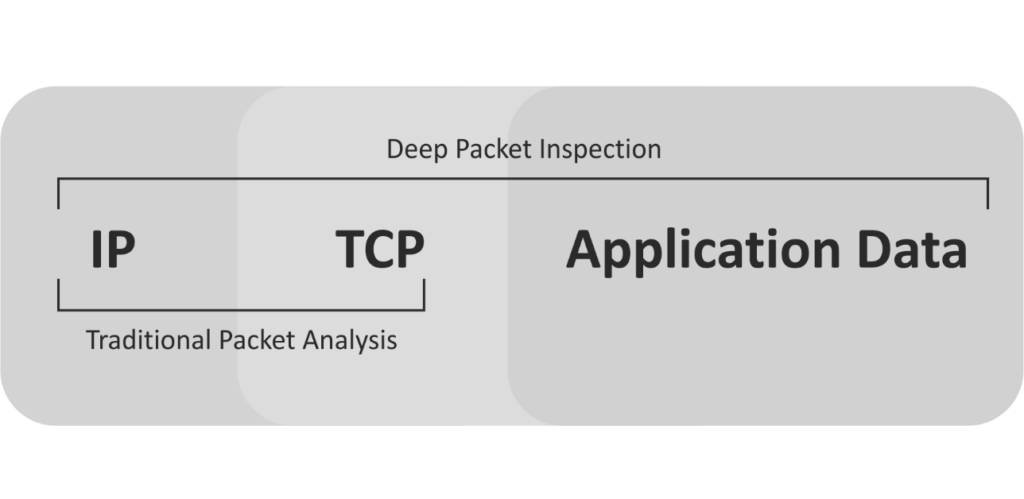
\includegraphics[width=0.75\textwidth]{img/DPI.png}
	\caption{Inspection area of DPI}
  \label{fig:dpiinspect}
\end{figure}
Deep Packet Inspection is a system for network packet filtering. It examines the data part (and often the header) of a packet as it passes an inspection point. 
As can be seen on \cref{fig:dpiinspect}, DPI examines the packet's data payload in depth as opposed to conventional packet filtering, which simply looks at the header section, allowing for more complex packet decision-making. DPI can detect, identify, classify, reroute, or prevent packets containing particular data or code payloads thanks to this sophisticated technique.

Due to its great versatility, DPI technology is employed in many different contexts, such as traffic management, censorship, eavesdropping, and network security. It is an essential tool for internet service providers and regulatory bodies since it can identify and manage apps using the network even in the face of encryption and port-hopping schemes.

\subsubsection{DPI in Relation to VPNs}
DPI is important when it comes to VPNs. In order to protect privacy and get around censorship or geographical limitations, VPNs usually encrypt data. Nonetheless, DPI can be used to examine encrypted packet metadata, including timing, size, destination, and protocol. This makes it possible to identify VPN activity even when the content is encrypted.

Certain DPI techniques can detect the signatures of the encryption protocols used by VPNs, allowing them to differentiate between conventional and VPN traffic. This capability is essential in situations when the use of VPNs is prohibited or closely watched, like in nations with severe internet censorship.

\subsubsection{DPI's Challenges for VPNs}
VPN technologies have substantial hurdles due to the efficacy of DPI:
\begin{itemize}
  \item \textbf{Detection and Blocking}: If Advanced DPI detects that a VPN is being used, it has the ability to either block or limit data, making the VPN useless for getting around censorship or geographical restrictions.
  \item \textbf{Avoiding Encryption}: Although DPI is unable to decrypt data, it can identify and potentially block VPN services based on educated estimates about the encrypted traffic's nature.
  \item \textbf{Adaptive Countermeasures}: VPN service providers are compelled to constantly modify and introduce fresh methods to avoid being detected by DPI, resulting in a never-ending game of cat and mouse between VPN providers and DPI-using companies.
\end{itemize}

\subsection{OpenVPN identification}
A first impression, may lead one to wonder how DPI systems are capable of differentiating between legitimate encrypted data such as secure HTTPS access to a website and VPN traffic. 
There are several techniques that DPI can use to identify OpenVPN traffic \citep{openvpn}:
\begin{itemize}
  \item \textbf{Protocol Signature Identification}: OpenVPN traffic can be recognized by DPI systems by looking for distinctive signatures in the packet headers. This is a conventional method that might work less well for OpenVPN because of its encryption and inconsistent port usage.
  \item \textbf{Heuristic analysis}: In this method, traffic patterns are examined to find traits common to VPN traffic, such as regular timing and packet sizes.
  \item \textbf{IP address and port inspection}: OpenVPN typically uses TCP or UDP port 1194, but it also has the option to use variable ports, which reduces the efficacy of this approach.
  \item \textbf{TLS Handshake Analysis}: VPN traffic, including OpenVPN, can be identified by examining the TLS handshake procedure, paying particular attention to the usage of particular cipher suites or TLS versions.
  \item \textbf{Timing and Packet Size}: DPI can identify consistent timing intervals and packet sizes in OpenVPN traffic.
  \item \textbf{Analysis of Encryption Patterns}: Even though OpenVPN encrypts its traffic, some encryption patterns might still be recognizable.
  \item \textbf{Behavioral Analysis}: VPN usage can be inferred by observing general network behavior, such as persistent, long-lasting connections.
  \item \textbf{Sequence Number and Acknowledgment Number Analysis}: Analyzing these numbers in TCP-based OpenVPN traffic can reveal VPN usage patterns.
  \item \textbf{Opcode Analysis in Packets}: the first 10 packets of a communication can be used as statistical characteristics for early detection of OpenVPN tunnels. By using the five bits of opcode in each packet to classify different types of packets.
\end{itemize}
These sophisticated methods, which focuses on statistical traits and traffic fingerprints, especially the opcode analysis, are very successful in identifying OpenVPN traffic, with low false positive rates and high accuracy \citep{openvpn}. In this context, the goal of VPN obfuscation can be described as attepting to bypass detection by trying to render as many as possible of the above mentioned techniques, as ineffectual.


\subsection{Packet manipulation}
One of the most important tools for the design of hardware implementation for the DPI is the finite state machine. This system design, in certain cases, may be exploited by utilizing packet manipulation techniques like packet fragmentation. \citep{dpisurvey2}
These attacks are even more relevant in the context of secure network environments, where traditional intrusion detection methods are employed.

In order to avoid detection by DPI systems, the following techniques may be employed:
\begin{itemize}
  \item \textbf{Fragmentation and noise padding}: Harmful data is divided into smaller pieces and mixed in with "noise" data, which is random or irrelevant data that doesn't interfere with the payload's ability to function. The idea is to trick DPI systems into thinking the fragmented packets are harmless, since these systems usually look for patterns in data to identify malicious activity. The attackers can effectively mask the malicious content, preventing it from being identified and prevented, by fragmenting the data and adding noise. DPI systems may find it especially difficult to defeat this strategy since it requires them to precisely reassemble and examine all of the packets in order to find the harmful content that is hidden—a laborious and resource-intensive procedure. \citep{dpifragmentation}
  \item \textbf{TCB Creation Evasion}: The first SYN packet that opens a TCP connection is manipulated in this tactic. A false state is produced in the TCP Control Block (TCB) of the censoring system by changing specific fields in this packet. Actual data packets are able to evade filtering without being noticed because of this manipulation, which makes the censorship monitor think that the link is either nonexistent or has already ended. \citep{censorshipdetection}
  \item \textbf{Data Reassembly Evasion}: This method takes advantage of flaws in the way censorship systems put back together broken TCP segments. When pieces of data are sent purposely out of order or overlapping, it makes it harder for the filtering system to correctly put these pieces back together and analyze them. This means that private information can get through the system that blocks them without being found or stopped. \citep{datareassembly}
  \item \textbf{TCB Teardown Evasion}: This method employs deliberately constructed packets, such as RST (reset), RST/ACK (reset acknowledgment), or FIN (finish), to prematurely end the Transmission Control Block in the censoring system. This premature termination results in the censorship system ignoring any subsequent packets from that connection. Nevertheless, the client-server link remains operational, enabling uninterrupted data flow without any intervention from censorship. \citep{tcbbreakdown}
  \item \textbf{Resync and Desync}: In this approach, particular packets are transmitted in order to initiate a re-synchronization of the censoring system's transmission control block with the specific TCP connection. Following this, an out-of-window sequence packet is transmitted, which ultimately results in the desynchronization of the censorship system from the link that is actually being employed. It is possible for data packets to avoid detection and censorship as a result of this difference. \citep{tcpevasion}
\end{itemize}

These serve as an example of how packet manipulation methods are capable of bypassing DPI. However, it should be noted that these tactics are, by far, not consistently effective and require a fair amount of manual labor to discover the specific packet sendings order, degree of fragmentation or noise required to bypass the DPI, if at all possible. 

\subsection{Protocol obfuscation}
Protocol obfuscation refers to the strategies used to change or conceal the properties of internet protocols in order to escape detection, censorship, or intervention from third parties. This is especially crucial in situations when internet access is tightly controlled or limited. Obfuscation prevents data packets from being detected by filters or detection systems that depend on established protocol signatures or patterns.
\subsubsection{General Methods of Protocol Obfuscation}
\begin{itemize}
  \item \textbf{Randomization}: In order to hinder automated systems from identifying patterns, random elements are incorporated into the communication protocol. For example, it may be challenging for Deep Packet Inspection (DPI) to recognize the traffic as being part of a particular protocol when packet sizes or timing change. \citep{randomization}
  \item \textbf{Protocol Mimicry}: By transforming the traffic of one protocol into that of another, more widely used protocol (such as HTTPS), users are able to evade filters that target particular types of data. A VPN might make its traffic look like normal HTTPS traffic, for instance. \citep{mimicry}
  \item \textbf{Header Manipulation}: Systems that use header analysis can't figure out what the data bits are if the header information is changed or encrypted. Changing port numbers or encrypting the whole header are two examples of this. \citep{headers}
  \item \textbf{Traffic Pattern Masking}: This technique entails modifying the attributes of traffic, such as its quantity, frequency, or trajectory, in order to conceal its true nature. It can be especially efficient against systems that examine traffic patterns over a period of time. \citep{masking}
\end{itemize}
\subsubsection{Focused methods for practical use}
Cosidering the wide range of techniques available, the selection was limited to four specific methods for experimentation:
\begin{itemize}
  \item \textbf{Port Switching}: To get around port-based filtering systems, it's easy but effective to change the port of the VPN server. Numerous DPI systems are set up to either watch or restrict traffic on particular ports that are known to be utilized by VPNs. The VPN traffic can get around these filters by periodically switching the server port. This approach is a sensible option for experimentation because it is simple to use and evaluate. \citep{crawford}
  \item \textbf{Steganography}: Data concealment is the approach of encoding sensitive information within seemingly innocuous data. It entails hiding the communication within seemingly innocuous data streams, such video or picture streams, within the framework of internet protocols. Systems that aren't built to identify such advanced concealment strategies can be severely harmed by this. To learn how well obfuscation holds up against sophisticated DPI systems, experiments will be conducted with steganography. \citep{osisteg}
  \item \textbf{Geneva Automated Censorship Evasion}: Geneva is an innovative method that makes use of genetic algorithms to automatically look for new ways to circumvent censorship. Geneva has the capacity to keep one step ahead of censoring systems if it continues to evolve and adapt to the environment with ongoing action. In the subject of protocol obfuscation and censorship evasion, testing Geneva provides a chance to investigate the ways in which automated systems might make a contribution to the field. \citep{Geneva}
  \item \textbf{Encryption Tunneling (utilizing stunnel or shadowsocks)}: This solution involves encrypting the communication, making it impossible for DPI devices to examine the data packets' contents. Tools such as stunnel and shadowsocks are designed to conceal and obscure traffic, offering an extra degree of security. This strategy is especially useful in circumstances where DPI systems are powerful and capable of performing in-depth analysis. The use of these tools for experimentation can provide useful information about the effectiveness of encryption-based obfuscation approaches. \citep{shadowsocks2}
\end{itemize}

To summarize, the discipline of protocol obfuscation provides a variety of methods to avoid censorship and surveillance. The four selected approaches for experimentation - port switching, steganography, Geneva automatic censorship evasion, and encrypted tunneling - possess distinct advantages and cater to various aspects of obfuscation. Their choice to conduct experiments with these subjects is warranted due to their significance in modern situations when internet censorship and surveillance are becoming more advanced. 

\subsection{Case Studies}
There exist numerous real-life examples of DPI being deployed and used on a significant scale. Some of the most notorious being:
\begin{itemize}
  \item \textbf{The Great Firewall of China (GFW)}: China's Great Firewall is a very well-known real-life applications of DPI technology. Among other censoring tools, it uses advanced DPI techniques to identify and restrict VPN connections. VPN service providers frequently need to improve their techniques on a regular basis to avoid being detected. \citep{gfw}
  \item \textbf{Iran's Internet Censorship}: Especially during political turmoil, Iran's government use DPI to monitor and regulate internet traffic, including the detection and blocking of VPN usage. \citep{iran}
  \item \textbf{Corporate Network Management}: By keeping an eye out for unauthorised VPN use that might go around corporate security measures, DPI is utilised in a business context to guarantee security and compliance.
  \item \textbf{Russia's Telegram Ban}: Using DPI, Russia attempted to ban the messaging service Telegram. Telegram, however, circumvented this restriction using a variety of strategies, including VPNs, illustrating the continuous conflict between DPI implementation and VPN evasion approaches. \citep{russia}
\end{itemize}

DPI not only poses a serious threat to VPN technologies but also propels the ongoing development of VPN obfuscation strategies including port switching, network steganography, and sophisticated tunnelling methods like Geneva, Shadowsocks, and Stunnel.

\subsection{Early DPI Evasion Methods}
Online security and privacy were issues that only a small minority of people worried about in the early days of the internet. But as digital technology developed, so did the techniques for keeping an eye on and filtering online behavior. Deep Packet Inspection started to spread widely and revolutionized the way that institutions and governments could monitor and regulate internet traffic. At first, it was possible to avoid DPI by utilizing networks like Tor or non-standard protocols. However, as DPI technologies advanced, these strategies encountered more difficulties, prompting creative solutions like Tor bridges. \citep{sechist}
\subsubsection{Rise of DPI and Intial Evasion Tactics}
Since Deep packet inspection goes farther than conventional packet filtering by checking the data part (content) of packets as they pass, rather than only the header. Governments and ISPs were able to regulate and control internet traffic with an unparalleled level of precision.

Many people, concerned about their right to privacy and freedom of expression, sought out ways to circumvent DPI as it gained traction. The use of non-standard protocols was one strategy. The original intention of DPI filters was to identify and regulate conventional internet traffic; however, users were able to circumvent these filters by employing less popular or custom-built protocols.

The Tor network was another effective solution against DPI. The Onion Router, or Tor for short, is a system that aims to hide one's online identity. It conceals the user's location and activity from network monitors by rerouting their web traffic through a network of relays. At first, it may like seemed to be a reliable way to avoid DPI—simply connect to Tor and use it. The traffic looked like typical encrypted web traffic.

\subsubsection{Advancement of DPI technologies}
But things started to change as DPI tools got better. DPI systems got smarter and could look at more protocols and even decrypted traffic trends. They started to notice the signs of Tor activity and the use of non-standard protocols, which made these ways of hiding from surveillance less effective.

Long lists of known IP addresses for Tor relays and entry nodes started to be used. They could stop the Tor network or keep an eye on people who tried to use it with these lists. Advanced DPI systems were also able to recognize Tor's unique traffic patterns, such as its uniform packet sizes and timing. So, using Tor or other obscure methods was no longer a surefire way to get around DPI.\citep{torblocking}

In response to these developments in DPI, the Tor Project created additional ways to assist users in maintaining their anonymity while still gaining access to the network. The introduction of Tor bridges was one of the those ways.

Tor bridges are alternate Tor network entry points that are not included in the public Tor directory. Because of this obscurity, they are less likely to be blocked or monitored than conventional Tor relays. Users in countries where the internet is strictly censored could use these bridges to connect to the Tor network without drawing attention to themselves.

Furthermore, the Tor Project launched pluggable transports, a technique meant to change the look of Tor traffic, making it difficult for DPI systems to recognize. Obfsproxy (obfuscated proxy), for example, disguises Tor traffic as conventional, innocuous-looking internet traffic. This makes DPI detection much more difficult. \citep{bridges}

Meek, another pluggable transport, employs a method known as domain fronting to make Tor traffic appear to be connecting with a prominent website such as Google or Amazon. This strategy takes use of the fact that restricting traffic to these important sites would cause enormous collateral harm, rendering censorship an unfeasible choice. \citep{domainfronting}

\subsubsection{The Ongoing Cat-and-Mouse Game}
The progression of DPI and the accompanying advancements in Tor technology symbolize an ongoing struggle between surveillance parties and proponents of internet privacy. As the technologies for DPI become more sophisticated, the techniques for circumventing them also become increasingly more complex. The implementation of Tor bridges and pluggable transports serving as a valid example of this continuing conflict.

Nevertheless, the usability of these approaches may differ depending on the geographical area and the particular DPI technology being employed. Tor bridges and other obfuscation techniques remain effective for evading detection in certain regions. In some cases, particularly in countries with sufficient government funding for advanced Deep Packet Inspection  technologies, even these advanced methods encounter difficulties. \citep{chinator}

\subsection{Modern DPI techniques}
Recent studies have taken an in-depth examination of the latest techniques employed by the Great Firewall of China to identify and prevent fully encrypted internet traffic. The main techniques are as so \citep{gfw}:
\begin{itemize}
  \item \textbf{Heuristic Rules for Exemption}: Based on the assumption that some types of traffic are unlikely to be fully encrypted, the GFW uses a set of heuristic rules to exempt them from blocking. This includes the fraction, position, and maximum contiguous count of ASCII characters; a rough entropy test based on the fraction of bits set; and rules based on common protocol fingerprints.
  \item \textbf{Entropy-Based Blocking}: The GFW denies access to connections based on the entropy of the client's initial TCP payload. As a sign of encrypted data, connections with a specific range of bits set per byte are blocked.
  \item \textbf{Exemption for ASCII Characters}: If the first six bytes are printable, more than half of the bytes are printable, or more than 20 consecutive printable bytes are present, the GFW will not block connections related to ASCII characters in the payload.
  \item \textbf{Protocol Exemptions}: Certain protocols—most notably TLS and HTTP—are specifically spared from blocking because their initial bytes match patterns that these protocols are known to use.
  \item \textbf{Blocking Mechanism}: The client's packets are dropped and never reach the server when the GFW detects encrypted traffic. This prevents further traffic from occurring.
  \item \textbf{Limited Scope and Probabilistic Blocking}: The GFW uses probabilistic blocking, which means that not all connections that satisfy the blocking requirements are obstructed. Blocking is purposefully restricted to particular IP ranges of well-known data centers.
  \item \textbf{UDP Traffic}: Sending UDP datagrams with a random payload does not result in blocking under the new censorship system, which is restricted to TCP.
  \item \textbf{Active Probing System}: Using a payload length-based rule in addition to similar rules, the GFW's active probing system operates in tandem with the traffic analysis system.
\end{itemize}

These methods highlight the GFW's sophisticated approach to censoring encrypted traffic while allowing standard internet communications. This aids in understanding the censorship mechanism and informs strategies to circumvent these blocks.

\subsection{Use of modern DPI techniques}
Since modern Deep Packet Inspection techniques have improved over time, effectively combating older methods used to evade such monitoring in the ever-changing world of internet restriction and spying, the capacity of authorities, such as those in charge of the Great Firewall of China, to identify and stop the many strategies that have historically been used to avoid censorship and surveillance has been greatly improved by recent developments in DPI technology.

\begin{itemize}
  \item \textbf{Advanced Signature Detection}: Older ways of getting around security measures often relied on hiding traffic signatures to look like allowed protocols or hide what kind of data was being sent. These days, DPI systems use more complicated algorithms that can better find trends and oddities in data packets. This includes being able to find small changes in how a protocol works, strange headers, and even patterns that could mean steganography or the use of hidden channels.
  \item \textbf{Behavioral Analysis and Anomaly Detection}: Newer DPI methods use behavioral analysis instead of just looking at the static features of traffic. This lets the systems figure out what normal network behavior looks like and spot changes that might be signs of attempts to get around the system. Anomaly detection algorithms can spot strange traffic patterns, like packet sizes that aren't normal, data amounts that don't match up, or unexpected use of protocols.
  \item \textbf{Machine Learning and AI Integration}: Adding Machine Learning (ML) and Artificial Intelligence (AI) to DPI systems is a big step forward in terms of what they can do. These technologies let the systems learn from the information they handle, which makes them better at finding things over time. In real time, AI algorithms can look at huge amounts of data and find complicated patterns and correlations that humans would never be able to see. \citep{dpiml}
  \item \textbf{Encrypted Traffic Analysis}: Many old DPI methods stopped working as much as encryption became more popular as a way to protect user privacy. Modern DPI methods, on the other hand, can look at encrypted data without having to decrypt it first. This is done by looking at statistics, time, and other side-channel data, which lets the authorities guess what kind of data is being encrypted.
  \item \textbf{Active Probing and Response Analysis}: These days' DPI systems don't just watch data; they also probe it and respond to it. These systems can figure out what kind of traffic or application is going on by sending specific packets or requests and looking at the replies. This works especially well against protocols that are made to look like other types of data.\citep{dpiprobing}
\end{itemize}
All of these DPI advacements have resulted in the slow yet noticable decline of non-modern DPI evasion methods. The most prevalent methods of evading DPI have been proxies and VPNs. The use of known VPN servers or IP addresses, as well as specific traffic patterns and handshake features, can be detected and blocked by modern DPI techniques.

Even anonymity networks like Tor, which aim to let users browse the internet anonymously and securely, are becoming more and more susceptible to DPI attacks. The unique features of Tor traffic, like packet timing and data transfer sizes, can now be detected by DPI systems, even when Tor employs obfuscation methods like pluggable transports.

Traditional methods of evading DPI also include obfuscation and Secure Shell (SSH) tunneling. Even when communication is disguised or contained within other protocols, contemporary DPI systems can still detect SSH based on its unique handshake and session features. \citep{sshtunneling}

Methods that masquerade as valid protocols (like HTTPS) in order to conceal harmful or restricted traffic are less successful when faced with current DPI. In order to distinguish between real protocol traffic and imposters, sophisticated algorithms examine time, packet size, and other subtle features. \citep{dpisslinspect}

Data packets' genuine nature might be concealed by using traffic fragmentation and padding, which were common techniques in legacy evasion strategies. In order to determine the true type or content of the traffic, modern DPI can reconstruct broken packets by analyzing the padding.
\section{Experimentation testbed}
When it comes to VPN encryption methods, building a virtual testbed is important for validating experimention results. This section is about the established testbed, including how it is set up, why certain tools were chosen, and how the network is structured overall. Vagrant and Libvirt were used to set up the testbed. These tools are essential for building and managing virtual machines (VMs) that mimic a real-world network environment so that VPN obfuscation methods can be tested.

An open-source software application, Vagrant allows to create and manage portable virtual environments for software development. It comes with a straightforward command-line client for controlling these settings, and a standard for configuration files to specify the virtual machines needed for a certain project. Because of its versatility, ease of use, and extensive support for several virtualization providers, including Libvirt, Vagrant was chosen for this testbed.

On the other hand, Libvirt presente withing itself a set of tools that can communicate with the virtualization features of newer Linux distributions (and other operating systems). As a management tool for platform virtualization, it is a C toolkit that interacts with Linux's virtualization features. The chosen choice for robust and scalable virtual networking experiments is due to its vast feature set and particularly well-known stability.

\begin{figure}[H]
	\centering
	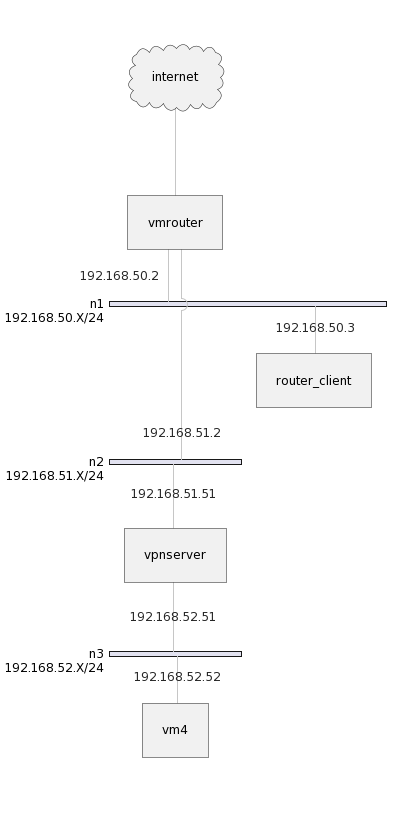
\includegraphics[width=0.6\textwidth]{img/topology}
	\caption{Testbed network topology}
  \label{fig:topology}
\end{figure}

The testbed consists of many virtual machines that are configured to imitate the major components of a VPN system as can be seen on \cref{fig:topology}, such as routers, VPN servers, and clients. The Vagrant configuration file defines four different VMs: vmrouter, routerslave, vpnserver, and vm4. Each VM is given unique network interfaces and IP addresses to ensure that it mimics the common network elements seen in a VPN situation.

The network topology was created to resemble a standard VPN environment with multiple network segments. The vmrouter acts as the primary router, connecting two different subnets. This VM is of course important as it simulates the gateway through which traffic is routed. The second VM, routerslave, is configured to act as a client to the router within the network, providing more realism to the client-server architecture commonly seen in VPN networks.

The VPN server is set up to be the vpnserver VM. This computer is very important to the testbed because it acts like the server side of a VPN. This is where different methods of encrypting data can be used and tried. The last VM, vm4, is a normal client in the network that is used to check how accessible and useful the VPN server is from the point of view of a client.

In some VMs, the network's dual-interface design lets for a complicated routing situation that works like a real VPN, where data traffic often goes through multiple network segments. This set-up is great for trying obfuscation methods that might be affected by different network paths and settings.


\subsection{Router Configuration}
The vmrouter virtual machine is an important part of the virtual network topology because it is meant to be a router in the Vagrant-based environment. This VM, which was set up using Vagrant with the "generic/ubuntu1804" box and provisioned for the libvirt provider, serves as a crucial node for network traffic management and routing in your VPN obfuscation method testing setup.

\subsubsection{Networking Interface Configuration}
\begin{table}[H]
	\caption{Network interfaces configuration on vmrouter}
	\centering
  \begin{tabular}{llllll}
\toprule
{} & Interface &       IP Address &    Subnet Mask & State &        MAC Address \\
\midrule
0 &        lo &        127.0.0.1 &      255.0.0.0 &    UP &  00:00:00:00:00:00 \\
1 &      eth0 &  192.168.121.216 &  255.255.255.0 &    UP &  52:54:00:02:6d:7a \\
2 &      eth1 &     192.168.50.2 &  255.255.255.0 &    UP &  52:54:00:a6:69:a2 \\
3 &      eth2 &     192.168.51.2 &  255.255.255.0 &    UP &  52:54:00:db:30:5d \\
\bottomrule
\end{tabular}
  \label{tab:vmrouter1}
\end{table}
The IP address \cref{tab:vmrouter1} shows that the vmrouter virtual machine has three network interfaces set up. Interfaces like as these are:
\begin{itemize}
  \item \textbf{eth0}: The subnet mask is 255.255.255.0 and the IP address is 192.168.121.216. This port serves as the main interface for communicating with the outside world, connecting the virtual machine to the network ouside the virutal topology.
  \item \textbf{eth1}: Set up with 192.168.50.2 as the IP address and 255.255.255.0 as the subnet mask. This interface is used for internal routing, and it's devoted to a private network.
  \item \textbf{eth2}: This interface, which shares the same subnet mask as eth1 and an IP address of 192.168.51.2, is to link to a separate part of the virtual network and performs internal routing in a similar fashion.
\end{itemize}
In order to manage and guide traffic within the virtual network, these interfaces are paramount. The setup points to a planned-out topology in which vmrouter is the central hub connecting various parts of the virtual environment.
\subsubsection{Routing Table Configuration}
\begin{table}[H]
	\caption{Routing table on vmrouter}
	\centering
\begin{tabular}{llllrrl}
\toprule
{} & Interface &    Destination &        Gateway &  Flags &  Metric &             Mask \\
\midrule
0 &      eth0 &        0.0.0.0 &  192.168.121.1 &      3 &     100 &          0.0.0.0 \\
1 &      eth1 &   192.168.50.0 &        0.0.0.0 &      1 &       0 &    255.255.255.0 \\
2 &      eth2 &   192.168.51.0 &        0.0.0.0 &      1 &       0 &    255.255.255.0 \\
3 &      eth0 &  192.168.121.0 &        0.0.0.0 &      1 &       0 &    255.255.255.0 \\
4 &      eth0 &  192.168.121.1 &        0.0.0.0 &      5 &     100 &  255.255.255.255 \\
\bottomrule
\end{tabular}
  \label{tab:vmrouter2}
\end{table}
The routing table for vmrouter is seen depicted in \cref{tab:vmrouter2}. 
\begin{itemize}
  \item Through the eth0 interface, 192.168.121.1 is established as the default gateway IP address for outgoing traffic. This indicates that this interface is the primary means by which data is sent to destinations outside the virtual network, to the internet.
  \item The fact that 192.168.50.0/24 and 192.168.51.0/24 are reserved for private networks shows that vmrouter uses the correct interfaces (eth1 and eth2) to route traffic intended for those networks.
\end{itemize}
By creating a barrier between internal and external network traffic, this configuration guarantees valid destination-based routing.
\subsubsection{Iptables Configuration}
\begin{table}[H]
	\caption{Iptables rules on vmrouter}
	\centering
\begin{tabular}{llllll}
\toprule
{} &        Chain &      Target &      Source &      Destination &  Additional Options \\
\midrule
0 &  POSTROUTING &  MASQUERADE &   0.0.0.0/0 &        0.0.0.0/0 &          -o eth0 -j \\
1 &  POSTROUTING &  MASQUERADE &   0.0.0.0/0 &  192.168.51.0/24 &          -o eth2 -j \\
2 &  POSTROUTING &  MASQUERADE &   0.0.0.0/0 &  192.168.50.0/24 &          -o eth1 -j \\
3 &      FORWARD &      ACCEPT &   0.0.0.0/0 &        0.0.0.0/0 &  -i eth0 -o eth1 -j \\
4 &      FORWARD &      ACCEPT &   0.0.0.0/0 &        0.0.0.0/0 &  -i eth1 -o eth0 -j \\
\bottomrule
\end{tabular}
  \label{tab:vmrouter3}
\end{table}
Based on how iptables is configured, vmrouter is also in charge of firewall rules and network address translation (NAT). The main points are as follows:
\begin{itemize}
  \item \textbf{MASQUERADE Rules:} These rules are set for all three interfaces (eth0, eth1, and eth2). The MASQUERADE target is used in to configure NAT. It allows outgoing traffic from the private network to appear as if it's coming from the vmrouter itself.
  \item \textbf{FORWARD Chain Rules:} The ACCEPT rules in the FORWARD chain for traffic going from eth0 to eth1 and back again show that vmrouter lets traffic go both ways between these interfaces. This is very important for a router that connects different network segments.
\end{itemize}


\subsection{Router Client Configuration}
The router\_client virtual machine is also an essential element in the network topology configuration. This virtual machine, labeled as "router\_client" , is setup to emulate a client within a network that interacts with a router and then later a VPN server. The router\_client VM's configuration demonstrates a setup that encompasses network interface settings, routing configurations, and script provisions to enhance setup and functionality.

\subsubsection{Networking Interface Configuration}
\begin{table}[H]
	\caption{Network interfaces configuration on router\_client}
	\centering
  \begin{tabular}{llllll}
\toprule
{} & Interface &       IP Address &    Subnet Mask & State &        MAC Address \\
\midrule
0 &        lo &        127.0.0.1 &      255.0.0.0 &    UP &  00:00:00:00:00:00 \\
1 &      eth0 &  192.168.121.199 &  255.255.255.0 &    UP &  52:54:00:71:5c:29 \\
2 &      eth1 &     192.168.50.3 &  255.255.255.0 &    UP &  52:54:00:7b:49:f2 \\
\bottomrule
\end{tabular}
  \label{tab:routerslave1}
\end{table}
As can be seen on \cref{tab:routerslave1} both eth0 and eth1 are set up as network interfaces in the router\_client virtual machine. Separate subnets are used to assign IP addresses to each interface. Both the eth0 and eth1 interfaces have the same subnet mask and IP addresses: 192.168.121.199 and 255.255.255.0, respectively. With its two interfaces, the virtual machine can link to two different networks, each of which represents a different part of the virtual network architecture.

The fact that eth1 has the private network address 192.168.50.3 suggests that it is part of a private network. The 192.168.50.0/24 subnet is for VM-to-VM communication, such as between the router\_client VM and vmrouter and other similar virtual machines. On the other hand, eth0's 192.168.121.199 IP address points to a separate portion of the network, which may be utilized for external communications or for connecting to a separate group of virtual devices or services however this eth1 interface has been rendered useless by the routing table configuration, in order to ensure all communication with other network devices happens through the vmrouter.

\subsubsection{Routing Table Configuration}

\begin{table}[H]
	\caption{Routing table on router\_client}
	\centering
  \begin{tabular}{llllrrl}
\toprule
{} & Interface &    Destination &        Gateway &  Flags &  Metric &             Mask \\
\midrule
0 &      eth1 &        0.0.0.0 &   192.168.50.2 &      3 &       0 &          0.0.0.0 \\
1 &      eth0 &        0.0.0.0 &  192.168.121.1 &      3 &     100 &          0.0.0.0 \\
2 &      eth1 &   192.168.50.0 &        0.0.0.0 &      1 &       0 &    255.255.255.0 \\
3 &      eth0 &  192.168.121.0 &        0.0.0.0 &      1 &       0 &    255.255.255.0 \\
4 &      eth0 &  192.168.121.1 &        0.0.0.0 &      5 &     100 &  255.255.255.255 \\
\bottomrule
\end{tabular}
  \label{tab:routerslave2}
\end{table}
Important information on the management and routing of traffic can be found in the router-\_client VM's routing table as shown on \cref{tab:routerslave2}. On the eth1 interface, the default gateway for the virtual machine is set to 192.168.50.2, which is the internal IP address of the vmrouter. With this configuration, all outgoing traffic from the router\_client VM will be sent to the vmrouter for additional routing decisions if no specified route has been configured.

The two network interfaces are also represented in the routing table. The 192.168.50.0/24 network is shown as a direct route for eth1, meaning that any traffic going to this subnet will be handled internally and won't require an external gateway. Similarly, eth0 handles traffic within this specific subnet as there is a direct link to the 192.168.121.0/24 network.

Moreover, a higher metric entry for the gateway 192.168.121.1 exists on eth0. Metric field indicates the cost of a route. The high metric is meant to make eth1 gateway the preferred route since it has the lower metric value.
\subsection{VPN Server Configuration}
Creating a flexible and functioning network architecture for testing VPN obfuscation methods is the primary focus of the configuration of the vpnserver virtual machine  in the virtual environment. This virtual machine, as stated before, is meant to act as a VPN server, which is a crucial component of a VPN network. The vpnserver VM's configuration includes network interface settings, routing configurations, and script provisions to enhance setup and functionality.

\subsubsection{Networking Interface Configuration}
\begin{table}[H]
	\caption{Network interfaces configuration on vpnserver}
	\centering
\begin{tabular}{llllll}
\toprule
{} & Interface &       IP Address &    Subnet Mask & State &        MAC Address \\
\midrule
0 &        lo &        127.0.0.1 &      255.0.0.0 &    UP &  00:00:00:00:00:00 \\
1 &      eth0 &  192.168.121.248 &  255.255.255.0 &    UP &  52:54:00:09:e7:27 \\
2 &      eth1 &    192.168.51.51 &  255.255.255.0 &    UP &  52:54:00:12:b1:b6 \\
3 &      eth2 &    192.168.52.51 &  255.255.255.0 &    UP &  52:54:00:8a:d6:81 \\
\bottomrule
\end{tabular}
  \label{tab:vpnserver1}
\end{table}
There are three network interfaces set up on the vpnserver VM as seen in \cref{tab:vpnserver1}: eth0, eth1, and eth2. Each of these ports is used for a different thing in the network setup:
\begin{itemize}
  \item \textbf{eth0:} The main interface that the VPN server uses to link to the outside world, created by default for the VM. Its subnet mask is 255.255.255.0 and its IP address is 192.168.121.248. This link is necessary to connect the VM to the outside world, which makes it easier to connect to the Internet and talk to people outside of the VM.
  \item \textbf{eth1:} This interface has an IP address of 192.168.51.51 and a subnet mask of 255.255.255.0. It is only used for interactions within the subnet connecting vpnserver and vmrouter.
  \item \textbf{eth2:} This interface is also used for internal network transmission, but on a different subnet to vm4, making it so only vpnserver has direct access to vm4. Which will be necessary for the testing of the VPN server.
\end{itemize}

\subsubsection{Routing Table Configuration}
\begin{table}[H]
	\caption{Routing table on vpnserver}
	\centering
\begin{tabular}{llllrrl}
\toprule
{} & Interface &    Destination &        Gateway &  Flags &  Metric &             Mask \\
\midrule
0 &      eth0 &        0.0.0.0 &  192.168.121.1 &      3 &     100 &          0.0.0.0 \\
1 &      eth1 &   192.168.50.0 &   192.168.51.2 &      3 &       0 &    255.255.255.0 \\
2 &      eth1 &   192.168.51.0 &        0.0.0.0 &      1 &       0 &    255.255.255.0 \\
3 &      eth2 &   192.168.52.0 &        0.0.0.0 &      1 &       0 &    255.255.255.0 \\
4 &      eth0 &  192.168.121.0 &        0.0.0.0 &      1 &       0 &    255.255.255.0 \\
5 &      eth0 &  192.168.121.1 &        0.0.0.0 &      5 &     100 &  255.255.255.255 \\
\bottomrule
\end{tabular}
  \label{tab:vpnserver2}
\end{table}
The IP routing \cref{tab:vpnserver2} of the vpnserver VM provides critical insights into how network traffic is managed and routed through the VM. The table consists of several entries, each defining a specific route:
\begin{itemize}
\item The default route is the one that uses eth0 and has the following parameters: destination 0.0.0.0, gateway 192.168.121.1. It sends data packets to the public internet if they don't fit any of the other routing criteria.
\item Both 192.168.51.0/24 and 192.168.52.0/24 routes, with eth1's gateway set to 0.0.0.0 and eth2's set to 0.0.0.0, manage traffic within their respective subnets for internal network traffic. 
\item Another entry in the routing table is the one for the 192.168.50.0/24 network, which goes via 192.168.51.2 on eth1. This route is reserved for sending data packets to a different subnet so that virtual machines can communicate with one another.
\end{itemize}
\subsubsection{Iptables Configuration}
\begin{table}[H]
	\caption{Iptables rules on vpnserver}
	\centering
  \scalebox{0.85}{
\begin{tabular}{lllllll}
\toprule
{} &        Chain &      Target & Protocol &          Source &      Destination & Additional Options \\
\midrule
0 &  POSTROUTING &  MASQUERADE &      N/A &  192.168.0.0/24 &        0.0.0.0/0 &  -o eth0 -j \\
1 &  POSTROUTING &  MASQUERADE &      N/A &       0.0.0.0/0 &  192.168.52.0/24 &  -o eth2 -j \\
2 &      FORWARD &      TCPMSS &      tcp &  192.168.0.0/24 &        0.0.0.0/0 &  -p tcp -m tcp  \\
\bottomrule
\end{tabular}
  }
  \label{tab:vpnserver3}
\end{table}
In the case of the vpnserver, an important part of controlling and protecting network traffic is the iptables setup on the vpnserver virtual machine as depicted on \cref{tab:vpnserver3}. Network Address Translation rules, packet forwarding rules, and TCP maximum segment size settings are all part of it:
\begin{itemize}
\item MASQUERADE (POSTROUTING): The VM can transform the IP addresses of packets coming from the internal networks (192.168.0.0/24 and 192.168.52.0/24) since the MASQUERADE rules are configured for NAT. In order to manage traffic from several sources and make it appear as though it is originating from a single IP, this is necessary for the VPN server.
\item TCPMSS (FORWARD Chain): For packets coming from 192.168.0.0/24, the TCP maximum segment size is adjusted by the rule in the FORWARD chain. For VPN setups in particular, this improvement is essential to preventing fragmentation and enhancing speed. The default MSS for an Ethernet network with an MTU of 1500 bytes is 1460 bytes \citep{mtu}; if this rule is not followed, TCP connections may use this value. However, the effective MTU is decreased when a VPN is utilized since the VPN protocol introduces extra headers. Inefficiencies and possible connectivity problems could result from packet fragmentation or dropping if the MSS is not adjusted appropriately.
\end{itemize}

\subsection{Remote Client Configuration}
The last essential part is the virtual machine "vm4", also known as the remote client. In order to test different VPN scenarios, this machine is built to mimic a distant client in a network. Most notably this VM is used to test whether a VPN still works correctly after an obfuscation method was implemented and also remote client is the recipient of requests from the router client VM during testing for measuring latency and throughput.
\subsubsection{Networking Interface Configuration}
\begin{table}[H]
	\caption{Network interfaces configuration on vm4}
	\centering
  \begin{tabular}{llllll}
\toprule
{} & Interface &      IP Address &    Subnet Mask & State &        MAC Address \\
\midrule
0 &        lo &       127.0.0.1 &      255.0.0.0 &    UP &  00:00:00:00:00:00 \\
1 &      eth0 &  192.168.121.97 &  255.255.255.0 &    UP &  52:54:00:19:0e:09 \\
2 &      eth1 &   192.168.52.52 &  255.255.255.0 &    UP &  52:54:00:bf:1f:e6 \\
\bottomrule
\end{tabular}
  \label{tab:vm4_1}
\end{table}
As seen on the above \cref{tab:vm4_1}, the vm4 virtual machine has two network interfaces set up. The following are the interfaces:
\begin{itemize}
\item \textbf{Interface eth0}: Vagrant provides this as the default interface. IP address is 192.168.121.234 with the subnet mask 255.255.255.0, as seen in the IP address column. The ip route table indicates that the gateway for this interface, which is used to connect to the outside world, is set at 192.168.121.1.
\item \textbf{Interface eth1}: This interface is allocated the IP address 192.168.52.52 with a subnet mask of 255.255.255.0. It is configured in Vagrant as a private network (via vm4.vm.network "private\_network", ip: "192.168.52.52"). Within the virtual network structure, this interface is meant for internal network connections.
\end{itemize}
\subsubsection{Routing Table Configuration}
\begin{table}[H]
	\caption{Routing table on vm4}
	\centering
  \begin{tabular}{llllrrl}
\toprule
{} & Interface &    Destination &        Gateway &  Flags &  Metric &             Mask \\
\midrule
0 &      eth0 &        0.0.0.0 &  192.168.121.1 &      3 &     100 &          0.0.0.0 \\
1 &      eth1 &   192.168.52.0 &        0.0.0.0 &      1 &       0 &    255.255.255.0 \\
2 &      eth0 &  192.168.121.0 &        0.0.0.0 &      1 &       0 &    255.255.255.0 \\
3 &      eth0 &  192.168.121.1 &        0.0.0.0 &      5 &     100 &  255.255.255.255 \\
\bottomrule
\end{tabular}
  \label{tab:vm4_2}
\end{table}
\begin{itemize}
\item \textbf{Default Gateway (eth0)}: 192.168.121.1 is the gateway for the 0.0.0.0 default route. This suggests that this gateway is used to route any traffic that isn't intended for the local network.
\item \textbf{Local Network (eth1)}: Since 192.168.52.0/24's route is directly connected, vm4 can speak with other computers on the network without the use of a gateway.
\item \textbf{Additional Routes}: The machine's configuration for managing traffic on the eth0 interface is indicated by the routes connected to 192.168.121.0/24 and the particular IP 192.168.121.1.
\end{itemize}

\section{Experimentation Results}
Experimentation with VPN obfuscation approaches is explained in depth, along with the findings, in this section. To determine how well each approach performed in different contexts, it was subjected to extensive testing in a controlled environment.

Resistance to detection, latency, throughput, and client-server accessibility are all part of the comprehensive set of evaluation criteria. With practical uses like evading censorship, protecting personal information, or communicating securely in dangerous settings in mind, the goal is to weigh the pros and cons of each approach.

The section concludes with a comparative analysis. A detailed table summarizing the results of each VPN obfuscation method in comparison to the specified criteria is included in this analysis. In addition, this part presents a new approach to using the collected data to choose the best VPN obfuscation method for individual users and their unique situations.

\subsection{Method Evaluation Criteria}
\subsubsection{Detection Resistance}
The most important measure for VPN obfuscation is detection resistance. A simple yet effective way to evaluate the practicality of an approach, this criterion assigns a pass or fail grade to its efficacy. Obfuscating VPN traffic is primarily done to avoid detection by Deep Packet Inspection technologies. Therefore, obfuscation effectiveness is proportional to how well it masks VPN traffic from DPI devices.

Determining how resistant a VPN obfuscation approach is to detection is a complex task. The well-known network protocol analyzer Wireshark is one of the main tools used in this evaluation. For delving into the complexities of network traffic, it is an indispensable tool. We get a full picture of how DPI interacts with VPN data by combining Wireshark with nDPI, a powerful open-source DPI tool. To better comprehend the detection resistance of different obfuscation strategies, nDPI enhances Wireshark's capabilities and permits a more thorough examination of packet data.


It should be kept in mind that no obfuscation technique is foolproof. Methods that work now in the provided testbed may become obsolete in the near future due to the dynamic nature of internet surveillance. 
\begin{figure}[H]
	\centering
	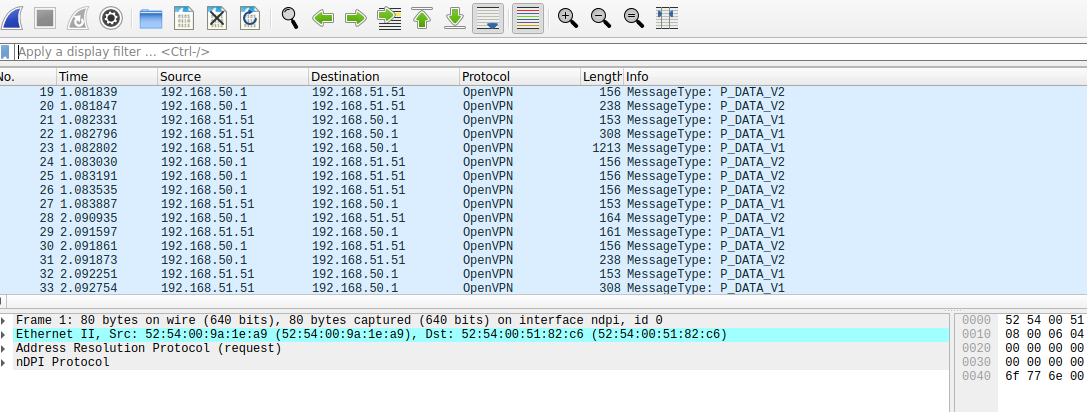
\includegraphics[width=1\textwidth]{img/before}
	\caption{WireShark capture of VPN traffic before obfuscation}
  \label{fig:before}
\end{figure}
\begin{figure}[H]
	\centering
	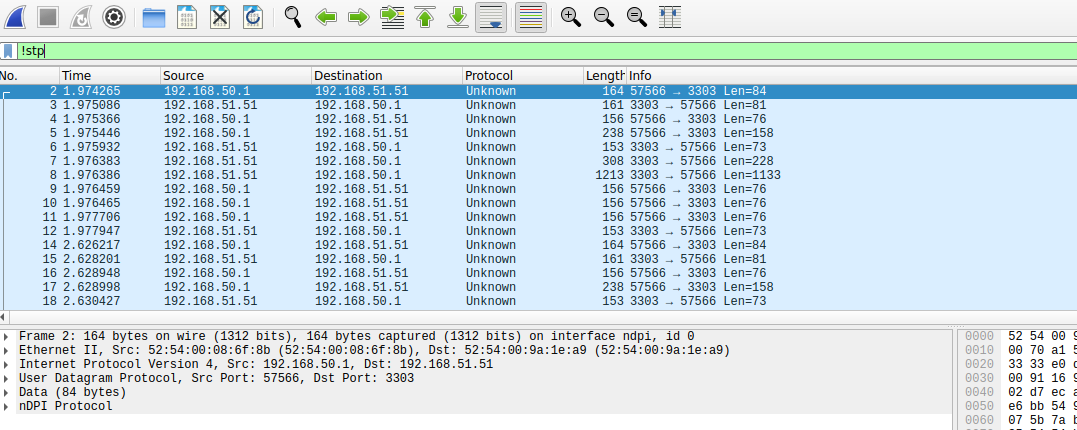
\includegraphics[width=1\textwidth]{img/after}
	\caption{WireShark capture of VPN traffic after obfuscation}
  \label{fig:after}
\end{figure}
The above \cref{fig:before} and \cref{fig:after} serve as an example of how the traffic looks like before and after successful obfuscation. The first image shows the traffic before obfuscation, and the second shows it after obfuscation. The traffic is identified to be OpenVPN in the first image, but it is completely unknown in the second. This is a good example of how a VPN obfuscation method should work.

\subsubsection{Latency}
The term "latency" describes the time it takes for a data packet to travel from its origin to its final destination. Usually, milliseconds (ms) are used to assess latency. Common methods for gauging network latency include the "ping" and "traceroute" commands, which track how long it takes for a packet to go from sender to receiver. However, since it is possible that ICMP requests are prioritized by an operating system, which would lead to the ICMP requests getting better latency results than what might be expected in real-life scenarios. As such, latency is tested by making a number of simple HTTP requests.

One of the most important metrics in network communications is latency, which is the amount of time it takes for a data packet to go from its origin to its final destination. Milliseconds (ms) is the standard unit of measurement for latency, which has far-reaching effects on the speed of network communications, the quality of the user experience, and the overall performance of systems in a wide range of applications, from basic web browsing to sophisticated real-time data processing.

Tools such as 'ping' and 'traceroute' are frequently used for measuring latency. The 'ping' command calculates the time it takes for a message to travel from its source to its destination. But 'ping' isn't perfect; different operating systems give varying priorities to ICMP requests, so the results could be deceiving. 

In my testing methodology, latency is assessed by making HTTP requests. This method is chosen to more accurately mimic the user's real-world interaction with the network. HTTP requests are a standard part of web browsing and online communications, thus providing a realistic measure of the latency that users are likely to experience.

\begin{figure}[H]
	\centering
	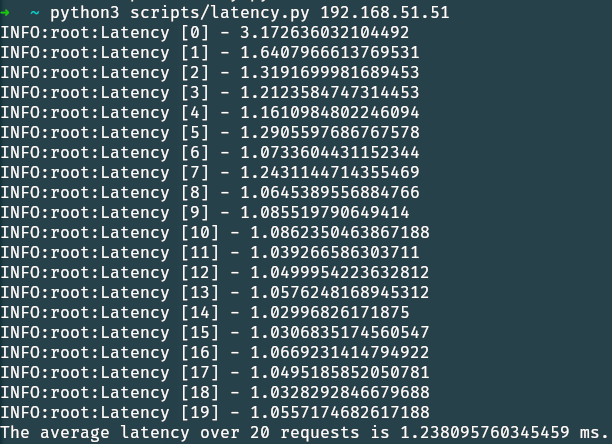
\includegraphics[width=0.8\textwidth]{img/latency}
	\caption{Latency test results}
  \label{fig:latency}
\end{figure}

\subsubsection{Throughput}
The amount of data successfully carried from one point to another within a particular time frame is represented by throughput, a crucial parameter in networking and computer systems. Bits per second (bps), kilobits per second (kbps), megabits per second (Mbps), and gigabits per second (Gbps) are typical units of measurement. A network's throughput—the rate at which data actually moves through the network—is a crucial performance indicator.

Though it may be noted that throughput and bandwidth are similar but different concepts. The real pace at which data may be moved over a network is known as throughput, whereas bandwidth is the theoretical maximum rate. Factors such as protocol overhead, packet loss, and network latency cause throughput to be lower than bandwidth. So in real-life, throughput is more helpful than bandwidth in determining network performance.

For measuting throughput the tool "iperf"" was utilized. 
It's an open-source program that works with most operating systems and has a command line interface. Iperf is a popular tool for testing and debugging network performance; it measures the maximum throughput a network can manage.
Two computers, a server and a client, need to be connected for Iperf to function. The Iperf client establishes a connection to the server and transmits data to it, while the Iperf server listens on a certain port. A brief overview of Iperf's usual usage is as follows:
\begin{itemize}
\item The first step in configuring Iperf is to choose a computer to function as the server and another to connect to the network. While clients initiate data transfers, servers listen for incoming connections.
\item After establishing a connection, the Iperf client starts transmitting data to the server. A number of parameters can be set to control this data transfer, including the test duration, the size of the data blocks, and the protocol (TCP in the latter case).
\item Measurement and Output: Iperf tracks the data transfer duration and amount. The system then computes the throughput and generates a performance report, showing the throughput's average and peak values throughout the testing time.
\end{itemize}
With Iperf's advanced features, users can test the network for jitter, packet loss, and duplex connection performance, among other things. 
The following figure gives a demonstration of the output Iperf generates:
\begin{figure}[H]
	\centering
	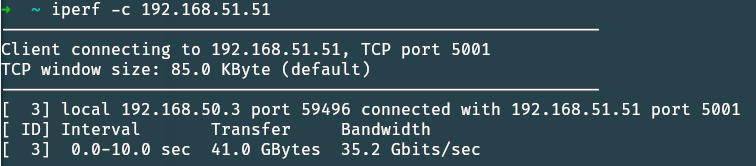
\includegraphics[width=1\textwidth]{img/iperf}
	\caption{Throughput test results}
  \label{fig:iperf}
\end{figure}


\subsubsection{Client-Server Accessibility}
Client-Server Accessibility can also be a crucial criteria depending on the circumstances. Most of the explored obfuscation methods require the user to access and make changes on the side of the VPN server, but if the user does not have access to the VPN server or is not allowed to make changes to it, this criteria becomes important. The ability of a VPN obfuscation method to be used without any changes to the VPN server is important to its success. The more accessible a method is to the client, the more likely it is to be effective in a real-world situation. This criteria is also boolean, meaning that a method either passes or fails.
\subsection{Port switching}
\subsubsection{Concept and Overview}
\subsubsection{Method Implementation}
\subsubsection{Evaluation}
\subsection{Steganography}
\subsubsection{Protocol Field Stegonagraphy}
\subsubsection{Multimedia Embedding Stegonagraphy}
\subsubsection{Method Implementation}
\subsubsection{Evaluation}
\subsection{Geneva}
\subsubsection{Concept and Overview}
\subsubsection{Method Implementation}
\subsubsection{Evaluation}
\subsection{Encryption tunneling}
\subsubsection{Concept and Overview}
\subsubsection{Method Implementation}
\subsubsection{Evaluation}
\section*{\centering Conclusion}

\addcontentsline{toc}{section}{Reference List}
\bibliography{refs.bib} % Entries are in the refs.bib file
\addcontentsline{toc}{section}{Appendix}
%
%\newcommand{\myappendix}[2]{}}

\clearpage
\vspace*{\fill}
\begin{quote} 
\centering 
\large \textbf{APPENDIX}
\end{quote}
\vfill % equivalent to \vspace{\fill}
\clearpage
\counterwithout{figure}{section}
\setcounter{figure}{0}

\captionsetup {
    format=customappendix,%
    labelformat=customappendix,%
    labelsep=custom
}

\renewcommand\mylstcaption{Example listing of code}

\newcounter{appcount}
\setcounter{appcount}{1}

%\begin{mdlisting}
%\begin{center} \textbf{Appendix \arabic{appcount}}\\ ./args.py \end{center}
%\lstinputlisting[language=python,basicstyle=\footnotesize]{/home/drewman/test/Nao-PPTX/src/args.py}
%\end{mdlisting}
%\stepcounter{appcount}

\begin{mdlisting}
\begin{center} \textbf{Appendix \arabic{appcount}}\\ ./slidepresentationservice.py \end{center}
\lstinputlisting[language=python,basicstyle=\footnotesize]{/home/drewman/test/Nao-PPTX/src/slidepresentationservice.py}
\end{mdlisting}
\stepcounter{appcount}

%\begin{mdlisting}
%\begin{center} \textbf{Appendix \arabic{appcount}}\\ ./services.py \end{center}
%\lstinputlisting,basicstyle=\footnotesize[language=python]{/home/drewman/test/Nao-PPTX/src/services.py}
%\end{mdlisting}
%\stepcounter{appcount}

\begin{mdlisting}
\begin{center} \textbf{Appendix \arabic{appcount}}\\ ./preader.py \end{center}
\lstinputlisting[language=python,basicstyle=\footnotesize]{/home/drewman/test/Nao-PPTX/src/preader.py}
\end{mdlisting}
\stepcounter{appcount}

\begin{mdlisting}
\begin{center} \textbf{Appendix \arabic{appcount}}\\ ./events/mediapresentationevent.py \end{center}
\lstinputlisting[language=python,basicstyle=\footnotesize]{/home/drewman/test/Nao-PPTX/src/events/mediapresentationevent.py}
\end{mdlisting}
\stepcounter{appcount}

\begin{mdlisting}
\begin{center} \textbf{Appendix \arabic{appcount}}\\ ./events/surveyevent.py \end{center}
\lstinputlisting[language=python,basicstyle=\footnotesize]{/home/drewman/test/Nao-PPTX/src/events/surveyevent.py}
\end{mdlisting}
\stepcounter{appcount}

\begin{mdlisting}
\begin{center} \textbf{Appendix \arabic{appcount}}\\ ./events/behavioractionevent.py \end{center}
\lstinputlisting[language=python,basicstyle=\footnotesize]{/home/drewman/test/Nao-PPTX/src/events/behavioractionevent.py}
\end{mdlisting}
\stepcounter{appcount}


\begin{mdlisting}
\begin{center} \textbf{Appendix \arabic{appcount}}\\ ./translation/texttranslator.py \end{center}
\lstinputlisting[language=python,basicstyle=\footnotesize]{/home/drewman/test/Nao-PPTX/src/translation/texttranslator.py}
\end{mdlisting}
\stepcounter{appcount}


%\begin{mdlisting}
%\begin{center} \textbf{Appendix \arabic{appcount}}\\ ./naoxml/xmlfinder.py \end{center}
%\lstinputlisting,basicstyle=\footnotesize[language=python]{/home/drewman/test/Nao-PPTX/src/naoxml/xmlfinder.py}
%\end{mdlisting}
%\stepcounter{appcount}

%\begin{mdlisting}
%\begin{center} \textbf{Appendix \arabic{appcount}}\\ ./naoxml/xmltag.py \end{center}
%\lstinputlisting[language=python,basicstyle=\footnotesize]{/home/drewman/test/Nao-PPTX/src/naoxml/xmltag.py}
%\end{mdlisting}
%\stepcounter{appcount}

%\begin{mdlisting}
%\begin{center} \textbf{Appendix \arabic{appcount}}\\ ./naoxml/xmltranslator.py \end{center}
%\lstinputlisting[language=python,basicstyle=\footnotesize]{/home/drewman/test/Nao-PPTX/src/naoxml/xmltranslator.py}
%\end{mdlisting}
%\stepcounter{appcount}

\begin{mdlisting}
\begin{center} \textbf{Appendix \arabic{appcount}}\\ ./comthread.py \end{center}
\lstinputlisting[language=python,basicstyle=\footnotesize]{/home/drewman/test/Nao-PPTX/src/comthread.py}
\end{mdlisting}
\stepcounter{appcount}

%\begin{mdlisting}
%\begin{center} \textbf{Appendix \arabic{appcount}}\\ ./general.py \end{center}
%\lstinputlisting,basicstyle=\footnotesize[language=python]{/home/drewman/test/Nao-PPTX/src/general.py}
%\end{mdlisting}
%\stepcounter{appcount}

\begin{mdlisting}
\begin{center} \textbf{Appendix \arabic{appcount}}\\ ./presentation.py \end{center}
\lstinputlisting[language=python,basicstyle=\footnotesize]{/home/drewman/test/Nao-PPTX/src/presentation.py}
\end{mdlisting}
\stepcounter{appcount}

%\begin{mdlisting}
%\begin{center} \textbf{Appendix \arabic{appcount}}\\ ./survey/survey.py \end{center}
%\lstinputlisting,basicstyle=\footnotesize[language=python]{/home/drewman/test/Nao-PPTX/src/survey/survey.py}
%\end{mdlisting}
%\stepcounter{appcount}

%\begin{mdlisting}
%\begin{center} \textbf{Appendix \arabic{appcount}}\\ ./main.py \end{center}
%\lstinputlisting,basicstyle=\footnotesize[language=python]{/home/drewman/test/Nao-PPTX/src/main.py}
%\end{mdlisting}
%\stepcounter{appcount}


\end{document}
# vim: set wrap:
